\section{Algoritmy}\label{sec:algorithms}

Počas vývoja výpočtovej techniky sa vyvíjali aj algoritmy pre kombinatorické hry, pričom piškvorky sú jednou z nich.
Tieto algoritmy je možné rozdeliť do 2 skupín: \emph{exaktné} a \emph{heuristické}; v tejto práci je popísaný jeden
algoritmus z každej skupiny.

\subsection{MiniMax}\label{subsec:algo-minmax}


Minimax je rozhodovacie pravidlo, podľa ktorého je možné určiť nasledujúci ťah.
Jeho princíp spočíva v maximalizovaní úžitku pre cieľového hráča a minimalizovaní úžitku pre oponenta.
Pôvodne bol vyvinutý pre \emph{hru s nulovým súčtom} (angl. zero-sum), čo je termín používaný v teórii hier. V
yjadruje hru, kde rozhodnutia hráčov sa dajú ohodnotiť nenulovým číslom $v$, pričom súčet za sebou idúcich hier má
súčet približne 0.
Často používaná hodnota je $v=1$ alebo $v=10$.
Ťah cieľového hráča je vyjadrený kladnou hodnotou ($+v$), ťah protihráča je vyjadrený zápornou hodnotou ($-v$) a remíza
je vyjadrená hodnotou $0$.
Hru, ktorú hrajú hráči striedavo, je možné vyjadriť pomocou postupnosti pre remízu:
\begin{equation}
    v-v+v-v+ \dots = \sum{v-v} = \sum{0} = 0
\end{equation}
(z čoho vychádza aj názov \emph{hra s nulovým súčtom}), resp. pre výhru jedného z hráčov:
\begin{equation}
    \pm v+v-v+v-v+ \dots = \pm v+\sum{v-v} = \pm v+\sum{0} = \pm v
\end{equation}
Rozhodovanie vychádza práve z tohto faktu, pričom algoritmus sa snaží nájsť takú postupnosť ťahov, ktorá by bola rovná
$+v$ (resp. maximálna), čo by znamenalo výhru cieľového hráča.
Samotný rozhodovací proces sa dá vyjadriť pomocou rozhodovacieho stromu vychádzajúceho z ktoréhokoľvek stavu hry.
Stavy hry tvoria vrcholy stromu a hrany predstavujú prechody medzi týmito stavmi.
Stav hry sa dá vyjadriť pomocou $d$-rozmernej tabuľky, kde hodnoty predstavujú \textbf{X}, \textbf{O} alebo prázdne
políčko.

Nech $l$ je maximálna výška rozhodovacieho stromu.
Ak nie je explicitne zadaná, potom maximálna výška stromu je počet voľných políčok vo východiskovom stave hry.
Nech $S_{ij}$ je stav hry, kde $i$ je úroveň stromu, v ktorom sa stav hry nachádza a $j$ je poradové číslo tohto vrcholu
v rámci úrovne $i$ určené pre jednoznačnú identifikáciu stavu hry a nech $p(S_{ij})$ je v strome rodič stavu $S_{ij}$
potom $\forall i, k, j \colon p(S_{i+1,k}) = S_{ij} \colon S_{i+1,k}$ vznikne vyplnením postupne každého
prázdneho políčka znakom hráča, ktorý je na ťahu na úrovni $i$.

Pre lepšiu predstavu je možné si situáciu ukázať na príklade z \hyperref[figure:minimax-tree]{nasledujúceho obrázku}.
Koreň stromu obsahuje 3 voľné políčka, jeho synovia vzniknú vyplnením postupne každého voľného políčka znakom hráča na
úrovni 2 (tzn. \textbf{X} na pozície 1. riadok, druhý stĺpec; tretí riadok, prvý stĺpec a tretí riadok, tretí stĺpec).
Takto sa naplní celý strom a jeho listy sa ohodnotia hotnotami $v$ pre víťazný stav hry, $-v$ pre prehru a $0$ pre
remízu (na \hyperref[figure:minimax-tree]{obrázku} vyznačené čiernou farbou).

Nech
\begin{equation}
    V(S_{ij}) =
    \begin{cases}
        \min{\{V(S_{i+1,j}) \forall j\}} & \text{ak v ťahu} i \text{je na ťahu protihráč} \\
        \max{\{V(S_{i+1,j}) \forall j\}} & \text{ak v ťahu} i \text{je na ťahu cieľový hráč}
    \end{cases}
\end{equation}
potom $\forall S_{ij}$ je priradená hodnota $V(S_{ij})$ pre $i = 1 \dots l-1$ a $\forall j$.
Najlepší ťah je potom určený spôsobom

\begin{equation}
    S_{Best} = \max{\{V(S_{2j}) \forall j \colon p(S_{2j}) = S_{11}\}} = \max{\{V(S_{2j}) \forall j\}}
\end{equation}

\begin{figure}[H]
    \centering
    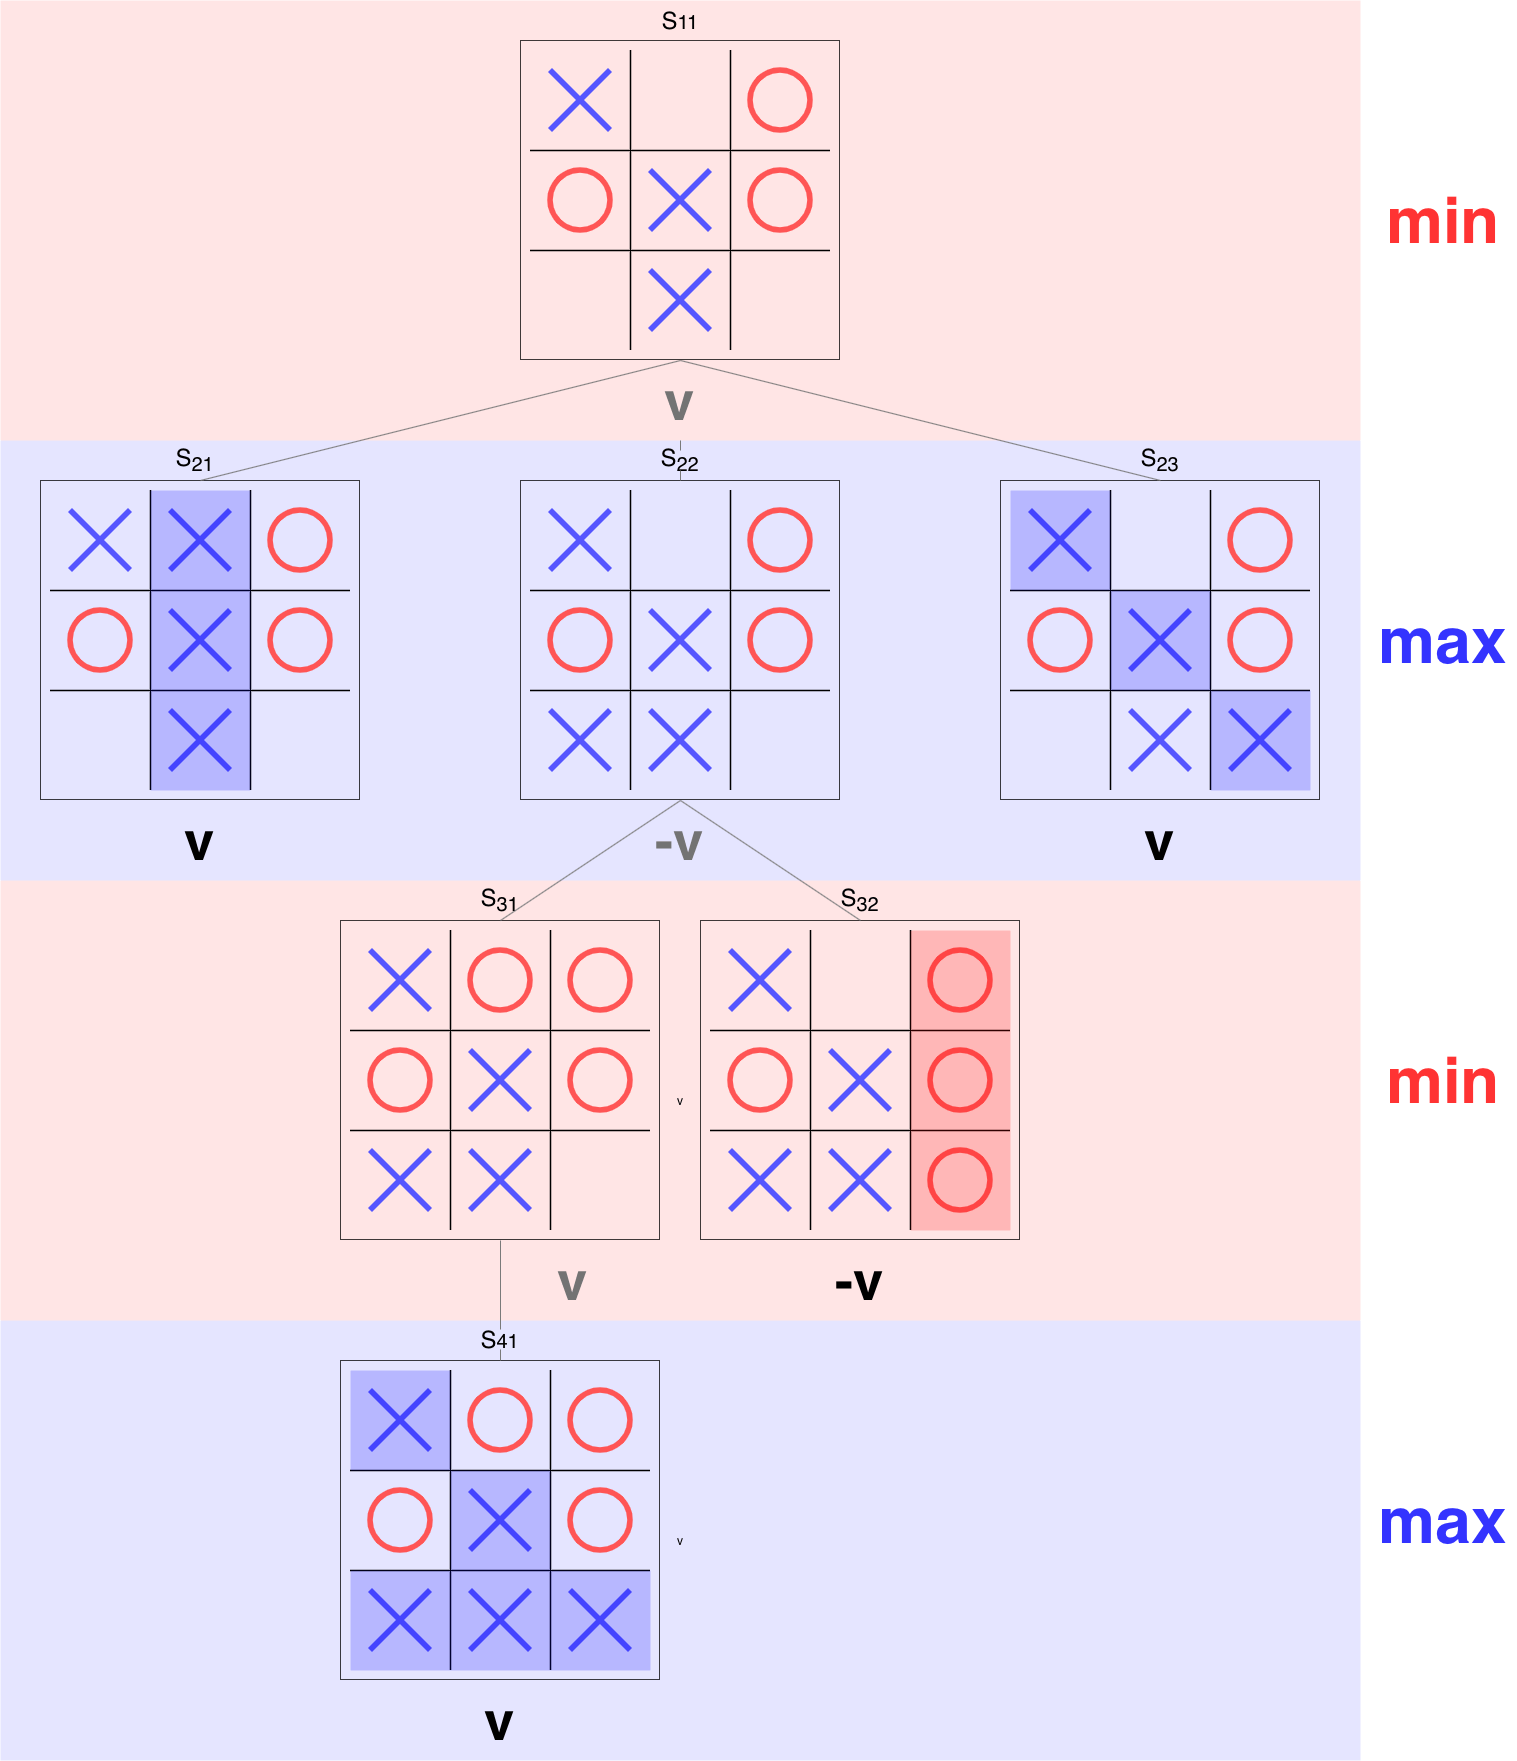
\includegraphics[width=0.8\textwidth]{images/minmax-tree.png}
    \caption{Rozhodovací strom algoritmu Minimax}
\end{figure}\label{figure:minimax-tree}

Algoritmus minimax patrí medzi \emph{exaktné algoritmy}, čo znamená, že pri hľadaní nájde najlepšie (optimálne)
riešenie, no prehľadáva všetky možné riešenia (celý vyhľadávací priestor).
Vo všeobecnosti pre neprázdne hracie pole o veľkosti $r$ v $d$-rozmernom hracom priestore s $o$ obsadenými políčkami je
možné veľkosť celého vyhľadávacieho priestoru vypočítať ako
\begin{equation}
    C(r, d, o) = (r^d - o) * (r^d - o - 1) * (r^d - o - 2) \dots 1 = \prod_{i = 1}^{r^d - o}{r^d - o - i + 1}
\end{equation}
Pre prázdne hracie pole (teda, kde $o = 0$) platí
\begin{equation}
    C(r, d, 0) = (r^d) * (r^d - 1) * (r^d - 2) \dots 1 = \prod_{i = 1}^{r^d}{r^d - i + 1}
\end{equation}

Ak algoritmus vychádza z prázdneho poľa o veľkosti $3 \times 3$ ($r = 3$, $d = 2$) je veľkosť vyhľadávacieho priestoru
$\prod_{i = 1}^{9}{10 - i} =$ \textbf{362 880}.
Na preskúmanie takéhoto počtu je možné použiť aj komerčnú výpočtovú techniku pričom výsledok bude známy v čase menšom
ako jedna minúta, no pri veľkosti $4 \times 4$ (teda $r = 4$, $d = 2$) je $C(4, 2, 0) \approx 2*10^{13}$ a čas
prehľadania priestoru sa (za predpokladu, že preskúmanie 1 možnosti trvá 1 milisekundu) zvýši na
\emph{$\approx 663$ rokov}.
Pre trojrozmernú plochu s rozmerom $3$ ($r = 3$, $d = 3$) je $C(3, 3, 0) \approx 1.08 * 10^{28}$, čo s rovnakým časovým
predpokladom znamená, že takýto výpočet by sa skončil po $\approx 3*10^{17}$ rokoch (pre predstavu: vek vesmíru sa
odhaduje na $\approx 14 mld. \approx 14 * 10^9$ rokov).

\subsection{Umelá neurónová sieť}\label{subsec:algo-ann}

Z vyššie uvedeného vyplýva, že exaktné riešenie pre väčšie rozmery plochy nie je možné použiť, teda je nutné použiť
algoritmy, ktoré nenájdu najlepšie riešenie v rámci celého vyhľadávacieho priestoru (optimálne), no vedia nájsť
najlepšie riešenie v rámci okolia východiskového riešenia (suboptimálne).
Takéto algoritmy sa nazývajú \emph{heuristické} a jednou z týchto heuristík je \emph{umelá neurónová sieť}.

\begin{itemize}
    \item na vstupe má byť aktuálny stav hry
    \item na výstupe má byť informácia o tom, ktoré pole je pre aktuálneho hráča najlepšie pre ďalší krok
\end{itemize}

Stav hry je reprezentovaný vektor $s_i$ pre $i=1 \dots r^d$, kde každých $r$ prvkov reprezentuje riadok hracej plochy,
resp. hracieho priestoru.
Napríklad pre rozmer 3x3 má vektor $s$ dĺžku 9 ($r^d=3^2$), prvky 1-3 reprezentujú prvý riadok, prvky 4-6 reprezentujú
druhý riadok a prvky 7-9 reprezentujú posledný riadok.
Neurónová sieť pozostáva z 3 vrstiev (vstupná, skrytá, výstupná).
Nech $x_i$ pre $i=1 \dots 3r^d$ je neurón vo vstupnej vrstve.
Za vstup do neurónovej siete je považovaný vektor hodnôt $x_1$ až $x_{3r^d}$, kde
\begin{equation}
    x_i=
    \begin{cases}
        1 & \text{ak }s_i\text{ je prázdne a } i \in \langle 1, r^d \rangle \\
        1 & \text{ak }s_{i-r^d}\text{ je }\textbf{X}\text{ a } i \in \langle r^d+1, 2r^d \rangle \\
        1 & \text{ak }s_{i-2r^d}\text{ je }\textbf{O}\text{ a } i \in \langle 2r^d+1, 3r^d \rangle \\
        0 & \text{inak}
    \end{cases}
    \quad
    \text{pre }i=1 \dots 3r^d
\end{equation}
Nech $y_j$ pre $j=1 \dots r^d$ je neurón v skrytej vrstve.
Táto vrstva zabezpečuje reprezentáciu stavu hry, na základe ktorej sa nastavujú váhy pre jednotlivé hodnoty políčok
hracej plochy.
Tieto váhy je možné označiť $w_{ij}$ pre $i=1 \dots 3r^d$, $j=1 \dots r^d$, kde index $ij$ vyjadruje váhu hodnoty
$x_i$ vstupujúcu do neurónu $y_j$.
Zo vstupnej vrstvy do skrytej vrstvy sa teda prenesú hodnoty
\begin{equation}
    \sum_{i=1}^{3r^d} w_{ij}x_{ij} \quad \text{pre } j=1 \dots r^d
\end{equation}
Posledná (skrytá) vrstva má len jeden neurón $z$, ktorý vyjadruje index $i$ vo vektore $s_i$ pre najlepší možný ťah
hráča.
Váhy zo skrytej vrstvy vstupujúce do poslednej vrstvy je možné označiť $v_j$.
Zo skrytej vrstvy do výstupnej vrstvy sa prenesú hodnoty
\begin{equation}
    \sum_{j=1}^{r^d} v_{j}y_{j}
\end{equation}
Neurónová sieť vyzerá nasledovne:

\begin{figure}[H]
    \centering
    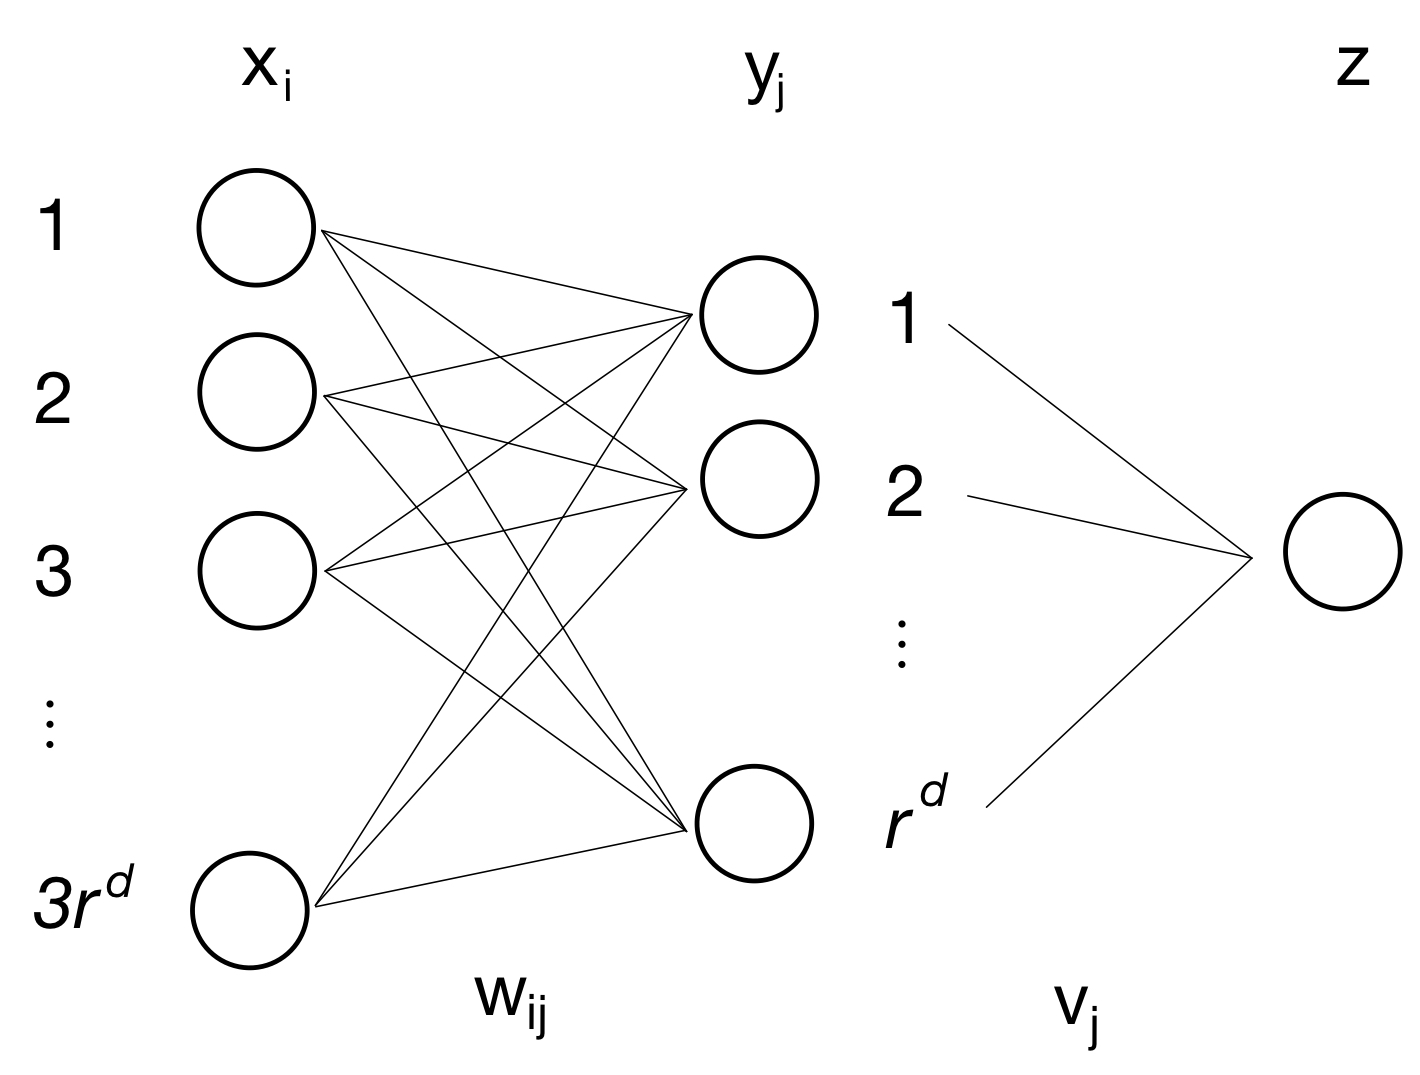
\includegraphics[width=0.5\textwidth]{images/ann.jpg}
    \caption{Návrh neurónovej siete}
\end{figure}

